\documentclass[11pt, letterpaper]{article}
\usepackage[utf8]{inputenc}
\usepackage[margin=1in]{geometry}
\usepackage{titlesec}
\usepackage{tabu}
\usepackage{enumitem}
\usepackage{amssymb}
\usepackage{graphicx}
\usepackage{caption}
\usepackage{listings}

\newlist{selectlist}{itemize}{2}
\setlist[selectlist]{label=$\square$,leftmargin=*,noitemsep,topsep=0pt}

\usepackage{hyperref}
\hypersetup{
    colorlinks=true,
    linkcolor=blue,
    filecolor=magenta,      
    urlcolor=cyan,
}
\urlstyle{same}

% Set up the section label formatting
\titleformat{\section}[block]{\hspace{1em}\bfseries}{\thesection.}{0.5em}{} 
\titleformat{\subsection}[block]{\hspace{1em}}{\thesubsection}{0.5em}{}
\titleformat{\subsubsection}[block]{\hspace{1em}}{\thesubsubsection}{0.5em}{}

% these are our own package-usages and declarataions; not part of the HardwareX template:
\usepackage{caption}
\usepackage{apacite}
\usepackage{eurosym}
\usepackage{abstract}
\DeclareCaptionType{equ}[][]
%----------------------

% no idention at the beginning of a new parahraph:
\setlength{\parindent}{0pt}

\title{Proteus - A Platform for Monitoring and Predicting Water Quality and Availability}
\author{Mika Engels, Ludwig M\"uller, Patrick Preu\ss{}, and Paul Sch\"utz}
\date{February 2020}


\begin{document}
\maketitle

\begin{abstract}
	We propose a hardware and software artifact which aims at helping to tackle Chile's ongoing agricultural water crisis. The artifacts combined allow for monitoring and predicting water quality and quantity.
	
	\smallskip
	\noindent \small \textbf{\textit{Keywords---}} water, monitoring, prediction, Chile, Arduino
	
	\smallskip
	\noindent \small \textbf{\textit{Affiliations---}} University of Cologne
	
	\smallskip
	\noindent \small \textbf{\textit{Contact email---}} mengels3@smail.uni-koeln.de, lmuell88@smail.uni-koeln.de, ppreuss1@smail.uni-koeln.de, pschuet5@smail.uni-koeln.de
\end{abstract}


\section{Hardware in Context}
\subsection{Motivation}
%TODO: Prediction einbauen
% Include a short description of the hardware, putting into context of similar open hardware and proprietary equipment in the field.
The access to drinking water is essential for human life as well as for life on earth in general. This and the mega drought Chile is facing in the near future requires the establishment of sustainable water usage in the entire country. Water resources, its distribution, and its usage in Chile is neither owned nor regulated nor controlled by a governmental institution. Rather there are several individual owners or communities in charge. Therefore, the installation of an appropriate monitoring system has the ability to improve the usage of water resources and gives all stakeholders of the drinking water industry an overall view over the resources. 
\newline

Any kind of such a system should be installed on a mandatory basis. The system has to be offered at a reasonable price especially for smaller, rural communities. The system has to measure some basic sensor data about wells. At least it measured the water level inside a well as well as its temperature and the pH value as a measure for quality. If required, the system could be extended with even more sensors, e.g. turbidity, but water level, temperature and pH value are always required. For transmission of sensor data, free radio networks like LoRaWAN is prefered. Such a radio network has not only the big advantage of being accessible freely but it also is easy to insall and has a great coverage going along with low energy consumption. A single gateway can cover an area up to 10km \footnote{https://www.tuv.com/media/corporate/products\_1/electronic\_components\_and\_lasers/\newline TUeV\_Rheinland\_Overview\_LoRa\_and\_LoRaWANtmp.pdf}. These gateways are configured to transmit the data received by the system installed at a well to a cloud instance where the data will be stored in an appropriate database. A platform will make this data then accessible for the well-owners as well as for the communities and population.
\newline

This gives the owners the possibility to have an overview over the changes in both quantity and quality of water resources. As already mentioned, a basic version of the system has to provide information about water level in a well and also the waters' temperature and pH value. It could also be useful to track incoming and outgoing water flows of the wells. Meanwhile, the population's advantage is basically that they can inform themselfes about the waters availability and qualilty they are using every day. In addition, these information help to protect the population from diseases caused by contaminated water.

\subsection{Related Work}
Environmental monitoring solutions have been designed and implemented before. Geetha and Gouthami categorize existing solutions along the following dimensions: whether the system is used to monitor running or stored water, whether it is deployed in- or outside (e.g. in a river or ocean), whether it monitors fresh water meant for drinking, and whether it allows to measure the quality of other environmental elements (e.g. air) as well \cite{geetha2016internet}. Monitoring systems whose sensors are located outside of buildings are most relevant to our design solution, as our hardware artifact should monitor the water in wells outside of buildings. For systems like this it has been shown that using multiple distributed wireless sensor networks based on low-cost internet of things (IoT) sensors yield the desired results regarding wide-area communication \cite{ingelrest2010sensorscope, geetha2016internet, jiang2009design, faustine2014wireless, zhenan2013sensor}.
\newline

The usage of sensors for measuring water-related quality data has been described for different use cases. The most commonly used sensors are sensors which measure the water's pH-value, its temperature, and its turbidity \cite{cloete2016design, jiang2009design, vijayakumar2015real, wiranto2015integrated}. Measuring water levels, which is highly relevant to our design solution (as it aims towards helping to tackle drought-related water shortages), has been implemented for dams \cite{siddula2018Dams, kavitha2018dams}, rivers \cite{amirruddin2012microcontroller}, and on agricultural land \cite{deekshath2018iot} before.
\newline

In the past, platforms that collect environmental data in large quantities have been created by governmental agencies and non-governmental initiatives alike \cite{mckinley2017citizen}. Most European and American countries enforce the collection of environmental data through their environmental protection agencies (e.g. Sweden\footnote{http://www.swedishepa.se/State-of-the-environment/Data-databases-and-applications/Environmental-monitoring-data/} or the United States\footnote{https://edg.epa.gov/data/}). As open as this data might be, it is not suitable for ad hoc visualization or real-time predictions, as most datasets published are snapshots at a single point in time. For communities that thrive to closely monitor their water resources, real-time data is needed. Non-governmental initiatives, especially so-called \textit{citizen science} projects, are an emerging source for different (including environmental) sorts of data \cite{kosmala2016assessing}.
\newline

The sensor-based systems described above usually include some means of alerting authorized personnel via cellular short message service or incorporate an online dashboard or some similiar kind of visualization for the gathered data \cite{shah2016customized}. Frameworks and algorithms for predicting data from wireless sensor networks have been developed and implemented as well, utilizing a variety of different statistical prediction methods \cite{wu2016data, mclean2005marine, lynch2008decentralized}.


\section{Solution Description}

The Proteus platform consists of three individual components. Namely those are the Proteusmeter, the Grafana dashboard, and the admin interface such as illustrated in Figure \ref{Architecture}. The Proteusmeter is an Arduino device with sensors which collects data about the well such as water level and water temperature and then forwards this data to our cloud server via LoRA network which then persists the sensor data. The Grafana dashboard provides an aggregated view of the collected sensor data and also provides basic forecasting functionality. This is the main point of contact for the communities and water agencies as it monitors the water levels and the water quality of all tracked wells. Furthermore there is an admin interface which allows the water agencies to add new wells or update exisiting wells. In the following chapters each component will be described in more detail.

\begin{figure}[ht!]
	\centering
	\includegraphics[width=120mm]{figures/architecture.png}
	\caption{Proteus Platform Architecture Overview \label{Architecture}}
\end{figure}

\subsection{Hardware Artifact}
The actual hardware device named Proteusmeter is basically an Arduino UNO REV 3 connected with several sensors and a combined LoRa/GPS shield ontop of the microcontroller. The Arduino and all sensor cablings are placed inside of a closed and waterproofed box with an incoming wiring harness for power supply and an outgoing wiring harness for sensors. The code running on the Arduino is a small programm written in an Arduino-specific language based on C and C++ and can be accessed via the GitHub repository\footnote{https://github.com/mengels3/proteus-platform/}. It reads the data from the sensors and transmits its via the LoRa-Shield.

\subsubsection{Hardware}
The basic version of a Proteusmeter contains three sensors: A water level sensor, a temperature sensor and a pH value sensor. The temperature and the pH value sensor have upstream controllers to convert the measured data to digital signals and therefore are connected to digital input ports at the Arduino. Their power supply is secured by the 5V and the 3.3V power supply ports of the Arduino UNO. Meanwhile, the water level sensor has its own power supply, its own circuit and is connected to an analog port of the Arduino. A basic Proteusmeter looks as shown in Figure \ref{Proteusmeter} in the real world. A schematic representation is shown in Figure \ref{schematic_Proteusmeter}. In the following all three sensors, their functionality and their wiring are described seperatly in detail.
\begin{figure}[ht!]
	\centering
	\includegraphics[width=120mm]{figures/box.jpg}
	\caption{An Proteusmeter and the three basic sensors \label{Proteusmeter}}
\end{figure}
\newline
\newline
\newline
\newline
\newline
\begin{figure}[ht!]
	\centering
	\includegraphics[width=160mm]{figures/Circuit.jpg}
	\caption{Schematic representation of a basic Proteusmeter \label{schematic_Proteusmeter}}
\end{figure}
\newline

The first and most important sensor is the water level sensor. It is a heavy metallic pole operating with 24 Volts power supply. Therefore the installation of an second power supply in addition to the supply of the Arduino is necessary. A transformator from 24V to 5V for the Arduino would be another option but is not that easy to realize and also more expensive. The Arduino measures the voltage at analog port A0 while a 220$\Omega$ resistor is connected in parallel to the Arduino. The high weight of the sensor presses the sensor to the ground of the well. The sensor measures the pressure difference between this point and the surface. The current surface pressure is measured via a small tube included in the cabeling. The higher the pressure difference is, the higher is the voltage present at the analog port of the Arduino. The analogRead()-function reads a raw value from 0 to 1023. Out of this raw value the actual voltage, the current, and finally the depth of the well can be calculated. The current is 4mA if the sensor is outside of the well. Every meter of depth increases the current by 3.2mA. The resulting formulas are:
\newline

\begingroup
\Large
%\begin{equ}
\begin{equation} 
Voltage [V]={\frac{raw\_value * 5 [V]}{1023}}
\end{equation}
\begin{equation} 
Current [mA]={\frac{Voltage [V] * 1000}{220 [\Omega]}}
\end{equation}
\begin{equation} 
Waterlevel [m]={\frac{Current [mA] - 4 [mA]}{3.2 [{\frac{mA}{m}}]}}
\end{equation}
%\caption{Equations to calculate water level \label{level-equation}}
%\end{equ}
\endgroup
\begin{figure}[ht!]
	\centering
	\includegraphics[width=60mm]{figures/water_lvl.jpg}
	\caption{Water level sensor \label{water_lvl}}
\end{figure}
\newline

The temperature sensor looks optically quite similar to the water level sensor even if it is much smaller and lighter. The placement depends on what will be most interesting for water agencies and could be at the gound of the well together with the level sensor or just below the water surface. In contrast to the level sensor this sensor can be supplied with the 3.3V port of the Arduino and does not need an own wiring circuit. It has its own upstream controller to transform the measured value into digital data. Therefore the sensor is connected to an digital port. With the digitalRead()-function the Arduino directly reads the current temperature in degree Celsius ($^{\circ}$C)
\begin{figure}[ht!]
	\centering
	\includegraphics[width=60mm]{figures/water_temp.jpg}
	\caption{Water Temperature Sensor \label{water_temp}}
\end{figure}
\newline

In contrast to both sensors described above the pH value sensor look and work different. Optically, the ph-probe is not a metallic but a plastic pole with a sensing area at the bottom. This sensor works with 5V power supply and has its own upstream controller to convert the measured values in digital data readable by the Arduino. But this sensor requires a connection to two digital ports of the Arduino. The Arduino reads a pH value as a string from the upstream controller. The sensor has to be calibrated occasionally. This can be done with three different liquids with specific pH values. The calibration source code can be downloaded from the manufacturer's website\footnote{https://www.atlas-scientific.com/product\_pages/kits/ph-kit.html}.
%In Addition to the ports used by the three sensors described the GPS shield needs two more digital ports. 
\begin{figure}[ht!]
	\centering
	\includegraphics[width=60mm]{figures/ph_value.png}
	\caption{Atlas Scientific pH Probe \label{ph_value}}
\end{figure}
\newline

\subsubsection{Software}
The source code running on the Arduino mircocontroller consits of four parts:
\begin{itemize}
	\item Reading pH value
	\item Reading and calculating values from water level and temperature sensor
	\item Querying GPS coordinates
	\item Sending all values as LoRa-Message
\end{itemize}
In the first part only the value of the ph probe is queried due to the sensors special characteristics. The full value is a string compounded from single characters received loopwise. The last character received is a newline (\textbackslash r). After this character a full pH value is received and returned by the respective function.
%\begin{lstlisting}
%	if (myserial.available() > 0) {                
%		char inchar = (char)myserial.read();
%		ph_value += inchar;
%		if (inchar == '\r') {
%			sensor_string_complete = true;
%		}
%	}
%\end{lstlisting}
\newline

After the pH value string reached this point the code continues with the next step. To determine the water level the formulas mentioned in the water level sensors's section are used: The raw value from analog port A0 is used in the first formula. From this point the level is calculated by using the result of formula (1) in formula (2) and the result of formula (2) in formula (3). For quering the temperature the package of the manufacturer has to be imported. Then the value in $^\circ$C can be read from a digital port.
%\begin{lstlisting}
%	raw_value = analogRead(A0);
%	voltage = (raw_value * 5.0) / 1023.0;
%	iamp = (voltage * 1000) / 220;
%	depth = (iamp-4) / 3.2;
%	
%	sensors.requestTemperatures(); 
%	temp = sensors.getTempCByIndex(0);
%\end{lstlisting}
\newline

The next step is the determination of the geographical position of the Arduino respectively the well. The GPS shield ontop of the Arduino delivers the current longitude and latitude. 
\newline

The last step is transmitting all values received from the sensors via LoRaWAN. The LoRa-Shield ontop of the Arduino is used for this purpose. A LoRa message (or LoRa-Package) consits out of a bunch of ``Key=Value''-Pairs seperated by semicolons. In Addition to the sensor values a device id is transmitted to assign the messages from different Arduinos. For transmitting the Message the package ``LoRa'' has to be included in the source code. After a settled delay the whole program starts again, queries the sensors again and transmits a new message.
%\begin{lstlisting}
%	LoRa.beginPacket();
%	LoRa.print("<");
%	LoRa.print(device_id);
%	LoRa.print(">device_id=");
%	LoRa.print(device_id);
%	LoRa.print(";level=");
%	LoRa.print(depth);
%	LoRa.print(";temp=");
%	LoRa.print(temp); 
%	LoRa.print(";ph=");
%	LoRa.print(ph_value);
%	LoRa.print(";long=");
%	LoRa.print(lon);
%	LoRa.print(";lat=");
%	LoRa.print(lat);
%	LoRa.endPacket();
%\end{lstlisting}


\subsection{Monitoring Platform}
The Proteusmeter monitoring platform is designed as a cloud-ready package of multiple small subsystems. It is made of four distinct parts: a database for storing measurement and master data, a dashboard that provides insight into the data, an API that is used to publish data, and an administrative interface. The monitoring platform can be deployed to a properly configured Infrastructure-as-a-Service (IaaS) or Platform-as-a-Service (PaaS) cloud environment as well as an on-premise solution, as it is distributed in pre-configured Docker\footnote{https://www.docker.com/products/container-runtime} container images.


\subsubsection{Data Publishing Interface}
To enable communities to gather data from a large fleet of Proteusmeter devices which may be spread across a long spatial distance, a wireless communication technology must be used. LoRaWAN\footnote{https://lora-alliance.org/about-lorawan} is used for Proteusmeters, because it is the most adopted one \cite{adelantado2017understanding}. A special LoRaWAN gateway device is used for (passively) collecting the sensor values from all devices in its range. The gateway has to be connected to the internet or a local area network, allowing it to transform the LoRa packages into ``ordinary'' transmission control protocol (TCP) packets. For this task, a small piece of software is running on the LoRaWAN gateway device itself, executing hypertext transfer protocol (HTTP) requests via a widely adopted network transfer library (cURL\footnote{https://curl.haxx.se/}), which allows the use of common security measures like transport layer security (TLS) encryption or certificate-based authentication methods.\footnote{There are many possible ways of authenticating a LoRaWAN gateway device: for instance see RFC5246 for details on client certificate authentication (https://tools.ietf.org/html/rfc5246\#section-7.4.4) or libssh's documentation on public-key-based challenge response authentication (http://api.libssh.org/master/libssh\_tutor\_authentication.html).}
\newline

In previous work on similar projects, researchers sent data packets like these to IoT data collection platforms like ThingSpeak\footnote{https://thingspeak.com/} or The Things Network\footnote{https://www.thethingsnetwork.org/}, from where they could be downloaded for analysis or visualization \cite{deekshath2018iot, sivaiah2018internet}. But the LoRaWAN gateway used for Proteusmeters rather sends all the data it receives to the application programming interface (API) of a custom web service. As a custom solution it (obviously) lacks the standardized APIs from well established platforms like ThingSpeak, but it allows for a maximum of flexibility regarding the data's structure and the volume of data transmitted.\footnote{While prototyping our artifacts, we found especially the latter one, volume of data transmitted, to be severly limited with the existing (openly accessible) IoT cloud platforms.} The API can be exposed publicly or could be hidden behind commonly used security means like a virtual private network (VPN). It allows for (almost) arbitrary environmental data to be published (see below), which greatly improves the future possibilities for Proteus as an environmental platform.
% REST API, (evtl Gateway, Tigerente?)

\subsubsection{Database} \label{sssec:database}
Proteus' cloud system by default comes equipped with a single PostgreSQL\footnote{https://www.postgresql.org/} database that stores all relevant data. The data can be categorized as (i) master data on the deployed wells and their location and sensors, as well as (ii) measurement data. The latter being the whole set of sensor values. These measurement data points are stored as key-value pairs, allowing for flexibility regarding the sensors canonical data type (floating point values vs. integer values vs. GPS coordinates etc.) as well as the actual database used. The default PostgreSQL instance could be swapped out for an non-relational database at any point without losing information.
% Database -> Postgres, ...

\subsubsection{Dashboard}
The main purpose for building the well sensor box is to collect data and provide a better overview on the current water situation in Chile. The sensors provide us with the ability to collect water from the wells, but in order to provide a monitoring for water shortages to the Chilean officials, a dashboard has to be developed. 
We persist the sensor data in a PostgreSQL database and use the open-source dashboarding platform Grafana to visualize the data. This dashboard will inform the official about water shortages or water contamination.
Grafana is an open-source dashboarding platform that offers a wide set of graphs and other panels one can place on their dashboard to visualize data. A plugin structure allows it to install even more third-party panels. Grafana is compatible to a large amount of data sources, which made it a perfect fit for the task at hand. 
To aggregate the data of several wells, the main dashboard page, contains a map showing all the wells connected to the platform and their water level. Additional panels show average information. A list of all the wells, can be used to jump to a more detailed dashboard for a dedicated well. On this detail view, the officials are able to analysis the development of water level, temperature, and pH value of a selected well. From this information you can derive whether the water is drinkable or not. The possibility to see a large time window, can help to better understand water shortages in certain areas of Chile.
\newline

\begin{figure}[ht!]
	\centering
	\includegraphics[width=12cm]{figures/Well_Inspection.png}
	\caption{Proteus Well Dashboard}
	\label{fig:grafana}
\end{figure}

To support the officials even more, a basic time-series prediction is included in the dashboard. On a separate dashboard page, one is able to see a prediction of our measured values. These predictions are based on the historic data from our database. A separate webservice endpoint offers this prediction using an AutoRegressive-Moving Average (ARIMA) model\cite{ARIMA}. ARIMA is stochastic model that can be used for a static time-series analysis. The ARIMA model looks for patterns inside the time-series data and tries to predict the next development of the curve. Using extensive weather data and by utilizing the grid structure of the wells one could build an even more advanced prediction. 

\subsubsection{Well Management Admin Interface}
The platform should enable the water agencies to add new wells and edit or delete exisiting wells dynamically. Therefore we provide an administrator interface where adminstrators can manage all wells. For example it could be the case that an existing well which currently only measures the water level gets an additional sensor for metering also the water temperature which can be considered a measure for water quality. In order for the system to know what type of parameter is actually measured and how it should display it we have to modify the existing well in the admin interface and add the temperature sensor to our well. This changes are directly stored to the database (see section \ref{sssec:database}). Figure \ref{fig:admin_interface_overview} shows a screenshot of the main interface where all wells are listed. When this figure was made apparently there were only two wells in our system. The first measured pH, temperature, and water level while the second measured only pH and temperature.
So this interface provides basic CRUD\footnote{Create,Read,Update,Delete} functionality for the well management.

\begin{figure}[ht!]
	\centering
	\includegraphics[width=16cm]{figures/admin_interface_overview.png}
	\caption{Proteus Well Management Admin Interface}
	\label{fig:admin_interface_overview}
\end{figure}

\section{Bill of Materials}
\tabulinesep=1ex
\begin{tabu} to \linewidth {|X|X|X|X|X|X|X|}
	\hline
	\textbf{Designator} & \textbf{Component} & \textbf{Number} & \textbf{Cost per unit currency} & \textbf{Total cost} & \textbf{Source of materials} \\\hline
	\textit{LoRa IoT Development Kit} & \textit{Dragino LoRa IoT Development Kit v2 868 MHz} & \textit{1} & \textit{124,95 \euro} & \textit{124,95 \euro} & \textit{EXP Tech}\\\hline
	\textit{Water Level Sensor} & \textit{TL231 DC24V 4-20mA Water Level Sensor} & \textit{1} & \textit{48,49 \euro} & \textit{48,49 \euro} & \textit{Amazon}\\\hline
	\textit{Water Level Sensor} & \textit{Aistuo 24V Power Supply} & \textit{1} & \textit{11,58 \euro} & \textit{11,58 \euro} & \textit{Amazon}\\\hline
	\textit{pH Probe} & \textit{Atlas Scientific Lab Grade pH Probe (Gen 2)} & \textit{1} & \textit{85,68 \euro} & \textit{85,68 \euro} & \textit{EXP Tech}\\\hline
	\textit{pH Probe} & \textit{EZO-pH Embedded pH Circuit} & \textit{1} & \textit{42,84 \euro} & \textit{42,84 \euro} & \textit{EXP Tech}\\\hline
	\textit{Water Temperature Sensor} & \textit{Velleman VMA324} & \textit{1} & \textit{13,99 \euro} & \textit{13,99 \euro} & \textit{Conrad}\\\hline
\end{tabu}


\section{Build Instructions}
%Provide detailed, step by step instructions for the construction of the reported hardware include all necessary information for reproducing the submitted hardware. Explain and, when possible, characterize design decisions. Including design alternatives if they exist. Use visual instructions such as schematics, images, and videos. Clearly reference design files and component parts described in the Design File Summary and Bill of Materials. Highlight potential safety concerns that may arise
The building of the Proteusmeter is done by the following steps:
\begin{itemize}
		\item Build the circuit required for the water level sensor and connect it with the Arduino
		\item Connect the upstream controllers of the temperature and the pH value sensors with digital Arduino ports
		\item Connect the pins of the GPS shield with digital Arduino ports
		\item Place the Arduino and the whole cabling inside an appropiate box
\end{itemize}
The basic instruction for all cablings were taken from the respective manuals. The whole sensor cabling (without the GPS cabling) is shown in Figure \ref{schematic_Proteusmeter} and has to be respected at all times.
\newline

The most difficult step is the circuit for the water level sensor. It is important to draw the circuit and think about voltages and currents before connecting the sensor with the power supply and especially the Arduino, because a higher voltage than 5V would destroy parts of the Arduino or more. This together with the information of an increasing current of 3.2mA for every meter of water depth the formulas provided in section 2.1.1 the required amount of resistance can be calculated and hence the whole circuit can be realized.
\newline

Since the other two sensors have upstream controllers for converting their signals into digital values the cabling is quite easy. For both sensors there are manuals how to use them correctly. An Arduino wiring manual for the temperature sensor can be found at the Arduino project hub\footnote{https://create.arduino.cc/projecthub/TheGadgetBoy/ds18b20-digital-temperature-sensor-and-arduino-9cc806}. For the pH probe the manufacturer's website is quite helpful\footnote{https://www.atlas-scientific.com/product\_pages/kits/ph-kit.html}. The same manuals also help to answer the question how to receive the sensor values at the software site. For the usage of the GPS shield it also has to get connected with digital Arduino ports. Again the manufacturer's website helps for cabling and at the software side of things\footnote{https://wiki.dragino.com/index.php?title=Lora/GPS\_Shield}.
\newline

The last step is the placement of the Arduino and the whole cabling inside of a closed and waterproofed box. This box needs two openings: At one side for both power supplies and at the other side for outgoing sensor cablings. In the closed state this box looks as shown in Figure \ref{Proteusmeter}. Uncovered it looks as in Figure \ref{unboxed_box}. As long as all intrcutions made in this section and by the manufacturer of the sensor are respected and the cabling are isolated appropiate there are no other electric security constrains.
\begin{figure}[ht!]
	\centering
	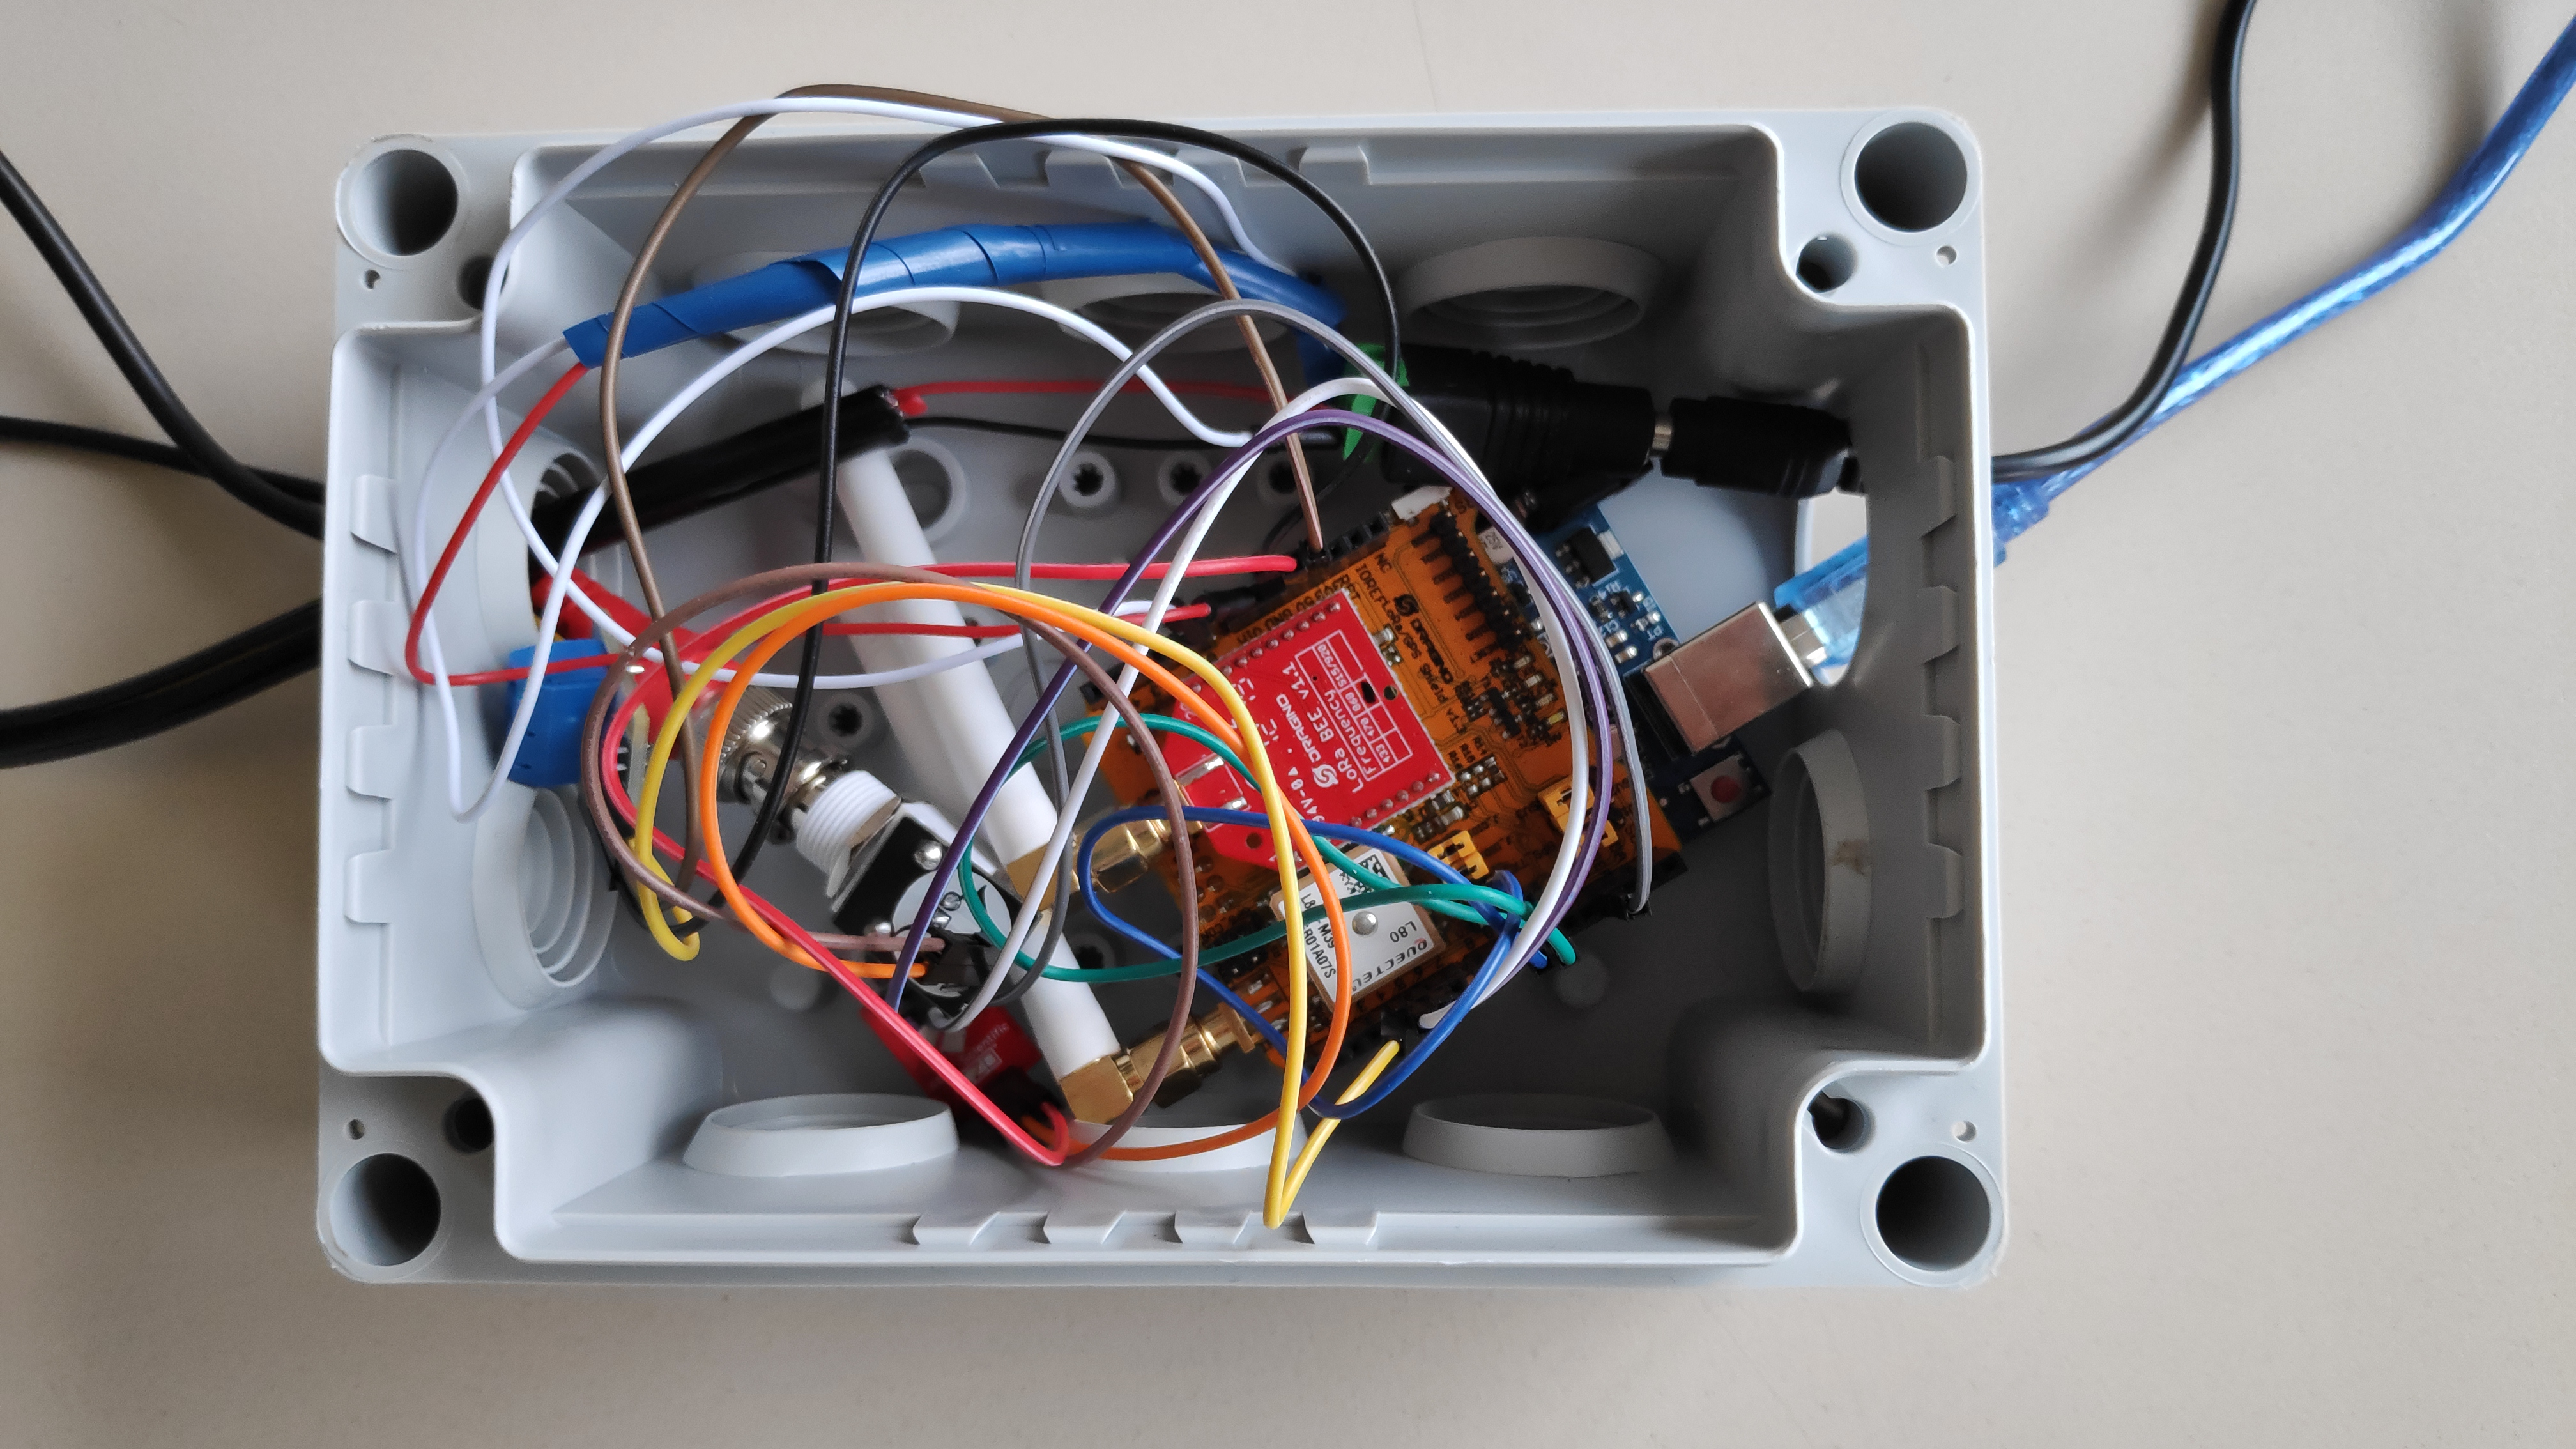
\includegraphics[width=160mm]{figures/box_unboxed.jpg}
	\caption{Inside of a Proteusmeter \label{unboxed_box}}
\end{figure}


\section{Operation Instructions}
In order to operate the Proteus platform and a set of Proteusmeters, the following steps must be taken. One has to
\begin{itemize}
	\item deploy the pre-configured Docker containers to a cloud system of their choice
	\item create a new entry for each well in the admin  interface, providing the appropriate data on its location, sensors etc.
	\item set up a LoRaWAN gateway device in a suitable spot where it covers the target area
	\item install the Proteusmeter boxes in all wells
\end{itemize}

The Docker images can be deployed to a cloud system or a single data center machine. If needed, the database implementation could be swapped out for a different one. Once the the images are deployed and all security measures are implemented (e.g. a VPN or a reverse proxy checking client certificates), a new well entity has to be created for each well that will be monitored by a Proteusmeter. It's not necessary to know all the wells and their values beforehand, these information can be fed or updated in multiple steps as well.
\newline

To be able to gather data from all Proteusmeters, one must find a suitable spot for a LoRaWAN gateway device, which not only allows for a good coverage of the targeted area, but also allows for a stable internet (or LAN) connection, as by default, data packets are only sent once. No retries are performed if data packets are lost. Once the gateway device is set in place, one has to adjust the data-transfer script (i.e. add a proper domain name or internet protocol address and configure any security measures like client certificate) and copy it to the gateway device. If necessary (e.g. due to the spatial distance that should be covered), more than one gateway could be deployed.
\newline

Last, the Proteusmeter boxes must be installed in the appropriate wells. The one who installs the boxes must ensure that the cable lengths matches the well's depth. For instance, the water level sensor described above must come with a cable long enough to reach the well's ground. Certain sensors (e.g. the pH value sensor described above) must be calibrated according to the manufacturers' specifications.


\section{Validation}
% Demonstrate the operation of the hardware and characterize its performance over relevant critical metrics .Demonstrate the use of the hardware for a relevant use case. If possible, characterize performance of the hardware over operational parameters. Create a bulleted list that describes the capabilities (and limitations) of the hardware. For example consider descriptions of load, operation time, spin speed, coefficient of variation, accuracy, precision and etc.
A first feasibility test was conducted during the initial development of the prototype. For this, DIN1401-compliant pipes were filled with water to simulate rising water levels in a well. The sensor data was then sent over a LoRa compatible radio frequency (868 MHz) to the LoRa gateway and from there it's send to the platform. Tests with the pH value sensor were done using citric acid. Adding the acid caused a significant drop of the reported pH value. The water level and temperature sensor were tested by pouring in hot water. This led to an increase of the measured temperature and the water level. These tests can ensure that all the sensor of the Proteus Box work properly and that the LoRa connection to the cloud works fine. 

\begin{figure}[h!]
	\centering
	\begin{tabular}{cc}
		\includegraphics[width=65mm]{figures/well_simulation1.jpg}
		\includegraphics[width=65mm]{figures/well_simulation2.jpg} \\
	\end{tabular}
	\caption{Well Setup}
	\label{fig:well_setup}
\end{figure}
\newpage

\section{Limitations and Future Work}
When prototyping the Proteusmeter device our laboratory setup was somewhat limited due to its laboratory nature itself. While aiming towards both a device and a platform that are as flexible as possible regarding the collection of arbitrary data, only so many different sensors could be used. We believe that the three sensors (i.e. for temperature, pH value, and water level) and the GPS coordinates combined are suitable as a proof of concept. Yet, expanding the Proteusmeter to use more (and different types of) sensors would be a reasonable direction for future work.
\newline

The Proteusmeter was also limited by its power supply and cable length, with the former being bound to an ordinary power outlet and the latter being rather short (less than 5m). Therefore, another direction could be to upgrade the Proteusmeter with a solar power panel, hydro generator or other kind of renewable energy source; or to test the device in a deep well, which would require longer cables and proper cable management (to avoid any debris, obstacles and the like).
\newline

A third possible direction for future work would revolve around the prediction of environmental phenomena, as our prototypical device only uses a single kind of prediction technique. Extending the predictive capabilities by more, different and more sophisticated prediction algorithms, the Proteus software artifact could be enhanced into a full-fledged environmental monitoring and prediction platform.

\section{Conclusion}
In this work we developed two artifacts that aim at helping communities in drought-stricken regions like rural parts of Chile to monitor their precious water resources. The piece of hardware we describe here is assembled from low-cost IoT-based sensors and a widely used microcontroller board. The low price of the parts used allows communities in rural areas to purchase them in large quantities and to deploy a large fleet of independent measurement devices.
\newline

The software artifact is an easy-to-use system for visualization and real-time predictions that is solely based on open-source technology. This and the pre-configuration of software container images, which allows for cost-efficient deployment in modern cloud environment, will help communities to keep the costs down as well. These two artifacts combined could help communities to not only gather knowledge on the status quo of their water resources. But also to better predict water shortages and act upon these information. Those communities willing to take one further step towards a federated environmental data platform could use the artifacts and the flexibility they provide to gain insight into even more environmental data.

%\section*{References}
\bibliographystyle{apacite}
\bibliography{literature.bib}
\appendix
\section{Group Assignment Overview Sheet}


\end{document}
